\documentclass[../main.tex]{subfiles}
\begin{document}

\begin{question}
    Exercise 3-1: Find all of the Nash equilibria and subgame perfect Nash equilibria of the following game.

    \centering
    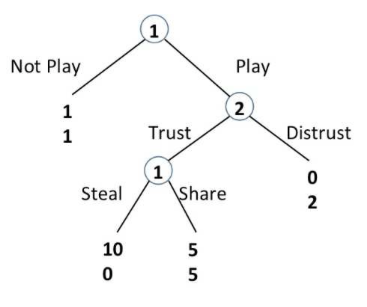
\includegraphics[width=0.4\textwidth]{Question3-1.png}
\end{question}

\begin{solution} 
\begin{itemize}
	\item Subgame perfect: $[(Not Play, Steal),(Distrust)]$
	\item Non subgame perfect: $[(Not Play, Share),(Trust)]$
\end{itemize}
\end{solution}

\begin{question}
Exercise 3-2: In a game where player $i$ has $N$ information sets indexed $n = 1, ..., N$ and $M_n$ possible actions at information set $n$, how many pure strategies does player $i$ have?
\end{question}

\begin{solution}
$\prod\limits_{n=1}^N M_n$
\end{solution}

\begin{question}
    Exercise 3-3: Rain\\
Players 1 and 2 must decide whether or not to carry an umbrella when leaving home. They know that there is a 50-50 chance of rain. Each player's payoff is -5 if she does not carry an umbrella and it rains, -2 if she carries an umbrella and it rains, -1 if she carries an umbrella and it is sunny and 1 if she doesn't carry an umbrella and it is sunny. Player 1 learns the weather before leaving home. Player 2 does not, but she can observe player 1's action before choosing her own
\begin{enumerate}
\item Write down the extensive form of this game as a game tree
\item Write down the induced normal form game.
\end{enumerate}
\end{question}

\begin{solution}
\begin{enumerate}
\item Game tree:
\begin{center}
\tikzset{
  % Two node styles for game trees: solid and hollow
  solid node/.style={circle,draw,inner sep=1.2,fill=black},
  hollow node/.style={circle,draw,inner sep=1.2},
}

% macro for entering payoffs
\newcommand\payoff[1]{
  $\begin{pmatrix} #1 \end{pmatrix}$
}

\begin{tikzpicture}[font=\footnotesize]
  \tikzset{
    level 1/.style={level distance=15mm,sibling distance=40mm},
    level 2/.style={level distance=15mm,sibling distance=20mm},
    level 3/.style={level distance=15mm,sibling distance=10mm},
  }

  \node[solid node,label=above:{N}]{}
  	child{node(r1)[solid node,label=left:{1}]{}
		child{node(rU)[solid node,label=left:{2}]{}
        		child{node[solid node,label=below:{\payoff{-2\\-2}}]{}
        			edge from parent node[left]{U}
        		}
            child{node[solid node,label=below:{\payoff{-2\\-5}}]{}
              edge from parent node[right]{NU}
            }
      		edge from parent node[left]{U}
      	}
      	child{node(rNU)[solid node,label=left:{2}]{}
            child{node[solid node,label=below:{\payoff{-5\\-2}}]{}
              edge from parent node[left]{U}
            }
            child{node[solid node,label=below:{\payoff{-5\\-5}}]{}
              edge from parent node[right]{NU}
            }
          edge from parent node[right]{NU}
        }
      	edge from parent node[left]{Rain (0.5)}
	}
	child{node(s1)[solid node,label=left:{1}]{}
    child{node(sU)[solid node,label=left:{2}]{}
            child{node[solid node,label=below:{\payoff{-1\\-1}}]{}
              edge from parent node[left]{U}
            }
            child{node[solid node,label=below:{\payoff{-1\\1}}]{}
              edge from parent node[right]{NU}
            }
          edge from parent node[left]{U}
        }
        child{node(sNU)[solid node,label=left:{2}]{}
            child{node[solid node,label=below:{\payoff{1\\-1}}]{}
              edge from parent node[left]{U}
            }
            child{node[solid node,label=below:{\payoff{1\\1}}]{}
              edge from parent node[right]{NU}
            }
          edge from parent node[right]{NU}
        }
        edge from parent node[right]{Sunny (0.5)}
  };

  \draw[bend left=15,-, dashed]  (rU) to node [auto] {} (sU);
  \draw[bend left=15,-, dashed]  (rNU) to node [auto] {} (sNU);
\end{tikzpicture}
\end{center}

\item Normal form game:
\begin{center}
	    \begin{tabular}{|l|c|c|c|c|}
	    \hline
	    			& $U_1 U$ 		& $U_1 NU$ 		& $NU_1 U$ 		& $NU_1 NU$ 	\\
	    \hline
	    $U_2 U$ 	& -1.5, -1.5 	& -1.5, -1.5	& -1.5, -2 		& 1.5, 2		\\
	    \hline
	    $U_2 NU$  	& -3, -1.5 		& -3, -3 		& -3, -0.5 		& -3, 2			\\
	    \hline
	    $NU_2 U$  	& -0.5, -1.5 	& -0.5, -0.5 	& -0.5, -3 		& -0.5, -2		\\
	    \hline
	    $NU_2 NU$  	& -2, -1.5	 	& -2, -2 		& -2, -1.5 		& -2, -2		\\
	    \hline
	    \end{tabular}
    \end{center}

\end{enumerate}
\end{solution}

\begin{question}
    Exercise 3-4: Investing smartly\\
Two players each invest \euro10 in a single long-term project that is executed in two phases. After each phase, the players have to simultaneously decide whether to withdraw their money from the project or not. If one or both of the investors pulls out after the first phase, the project has to shut down prematurely and only \euro12 can be recovered. After phase two, the project yields \euro30. After each phase, if both players withdraw, the money is divided evenly. If only a single player withdraws, she gets back her entire investment and, if applicable, all of the profits (the profit is \euro0 after round 1 and \euro10 after round 2). If none of the player withdraws their money after the second phase, they both receive \euro10.
\begin{enumerate}
\item Write down the extensive form game of this problem as a game tree.
\item Identify all Nash equilibria.
\item Identify all subgame perfect Nash equilibria.
\end{enumerate}
\end{question}

\begin{solution}
\begin{enumerate}
\item Game tree:
\begin{center}

\tikzset{
  % Two node styles for game trees: solid and hollow
  solid node/.style={circle,draw,inner sep=1.2,fill=black},
  hollow node/.style={circle,draw,inner sep=1.2},
}

% macro for entering payoffs
\newcommand\payoff[1]{
  $\begin{pmatrix} #1 \end{pmatrix}$
}
\begin{tikzpicture}[font=\footnotesize]
  \tikzset{
    level 1/.style={level distance=15mm,sibling distance=50mm},
    level 2/.style={level distance=15mm,sibling distance=20mm},
    level 3/.style={level distance=15mm,sibling distance=20mm},
    level 4/.style={level distance=15mm,sibling distance=10mm},
    level 5/.style={level distance=15mm,sibling distance=0mm},
  }

  \node[solid node,label=above:{1}]{}
  	child{node(3)[solid node,label=left:{2}]{}
        		child{node[solid node,label=below:{\payoff{6\\6}}]{}
        			edge from parent node[left]{W}
        		}
        		child{node[solid node,label=below:{\payoff{10\\2}}]{}
        			edge from parent node[right]{NW}
        		}
      	edge from parent node[left]{W}
	}
	child{node(4)[solid node,label=right:{2}]{}
            child{node[solid node,label=below:{\payoff{2\\10}}]{}
              edge from parent node[left]{W}
            }
        child{node[solid node,label=left:{1}]{}
        	child{node(1)[solid node,label=left:{2}]{}
            	child{node[solid node,label=below:{\payoff{15\\15}}]{}
              		edge from parent node[left]{W}
            	}
            	child{node[solid node,label=below:{\payoff{20\\10}}]{}
              		edge from parent node[right]{NW}
            	}
            	edge from parent node[left]{W}
            }
            child{node(2)[solid node,label=right:{2}]{}
            	child{node[solid node,label=below:{\payoff{10\\20}}]{}
              		edge from parent node[left]{W}
            	}
            	child{node[solid node,label=below:{\payoff{10\\10}}]{}
              		edge from parent node[right]{NW}
            	}
            	edge from parent node[right]{NW}
            }
          edge from parent node[right]{NW}
        }
        edge from parent node[right]{NW}
  };
   \draw[-, dashed]  (1) to node [auto] {} (2);
   \draw[-, dashed]  (3) to node [auto] {} (4);

\end{tikzpicture}
\end{center}

\item $[(W,*)$ $(W,*)]$ 
\item $[(NW,W)$ $(NW,W)]$\\ 
	$[( ,W)$ $( ,W)]$

\end{enumerate}
\end{solution}

\begin{question}
    Exercise 3-5: Piracy\\

In this exercise, we explore what would happen if pirates (ahrrrr) were not only treacherous, selfish and
thirsty for blood, but also extremely intelligent.
Five pirates have obtained 100 gold coins and have to divide up the loot. The captain proposes a distribu- tion of the loot. All pirates then vote on the proposal, and if half the crew or more go “Aye”, the loot is divided as proposed. If the captain fails to obtain support of at least half his crew (including himself), all pirates turn against him and make him walk the plank. The pirates then start over again with the next most senior pirate as captain. Obviously, each pirate prefers any outcome where he survives over any outcome where he dies. Given survival, each pirate wants to maximize the number of gold coins he receives. Given equal amounts of gold, each pirate prefers to throw as many pirates overboard as possible.
Let five pirates be $A,B, C, D$ and $E$ and assume a strict order of seniority where $A$ is more senior than $B$, $B$ is more senior than $C$ and so on. What are the subgame-perfect equilibria of this game?
\end{question}

\begin{solution}
$A > B > C > D > E$
\begin{itemize}
	\item $E$: 100 v
	\item $D$: (100, 0)
	\item $C$: (99, 0, 1)
	\item $B$: (99, 0, 1, 0)
	\item $A$: (98, 0, 1, 0, 1)
\end{itemize}
\end{solution}

\begin{question}
Exercise 3-6:
\end{question}

\begin{solution}
\end{solution}

\begin{question}
Exercise 3-7:
\end{question}

\begin{solution}
\end{solution}

\begin{question}
Exercise 3-8:
\end{question}

\begin{solution}
\end{solution}

\begin{question}
Exercise 3-9:
\end{question}

\begin{solution}
\end{solution}

\begin{question}
Exercise 3-10:
\end{question}

\begin{solution}
\end{solution}

\begin{question}
Exercise 3-11:
\end{question}

\begin{solution}
\end{solution}

\end{document}

